\section{Slow Feature Analysis}

  Slow feature analysis also another special case of a linear factor model that uses information from time signals to learn invariant features. It is motivated by a general principle called the \textbf{slowness principle}. The idea is that the important characteristics of scenes change very slowly compared to the individual measurements that make up a description of a scene. For example, in computer vision, individual pixels can change very rapidly. If a zebra moves from left to right across the image, an individual pixel wil rapidly change from black to white. By comparison, the feature indicating whether a zebra is in the image will not change at all, and the feature describing the zebra's position will change slowly. Therefore, we want to regularize our model to learn features that change slowly over time.  

  We can apply the slowness principle to any differentiable model trained with gradient descent. That is, we can add the following term to the loss function: 
  \begin{equation}
    \lambda \sum_i d\big( f(x^{(t+1)}), f(x^{(t)}) \big)
  \end{equation}
  where $\lambda$ is a hyperparameter determining the strength of the slowness regularization term, $t$ is the time index, $f$ is the feature extractor to be regularized, and $d$ is the distance between $f(x^{(t)})$ and $f(x^{(t+1)})$. A common choice for $d$ is the mean squared difference. 

  Essentially, given a set of time-varying input signals $x^{(t)}$, SFA learns a nonlinear function $f$ that transforms $x$ into slowly-varying output signals $y$. Obviously, we can't just take some trivial function like $f = 0$, so we have the following constraints 
  \begin{align}
    \mathbb{E}_t [ f(x^{(t)})_i]  & = 0 \\ 
    \mathbb{E}_t [ f(x^{(t)})_i^2] & = 1 
  \end{align}
  \begin{center} 
    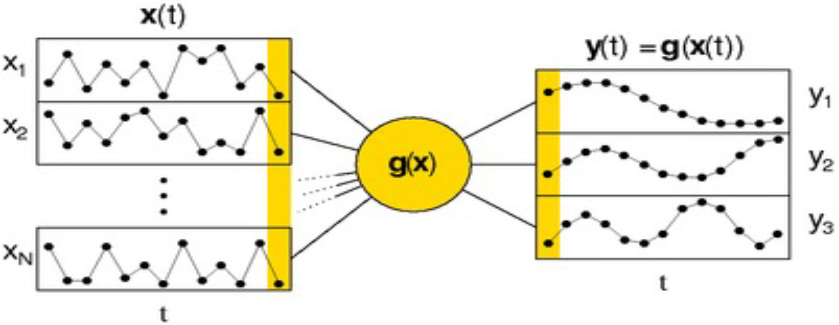
\includegraphics[scale=0.4]{img/slow_feature.png}
  \end{center}
  We can restrict the nonlinear $f$ to some subspace of functions, and this becomes a standard optimization problem where we solve 
  \begin{equation}
    \min_\theta \mathbb{E}_t \big[ \big( f(x^{(t+1)})_i - f(x^{(t)})_i \big)^2 \big]
  \end{equation}

